%\subsection{Histogramm f\"ur Evaluation Method (188)}
%\begin{figure}
\begin{center}
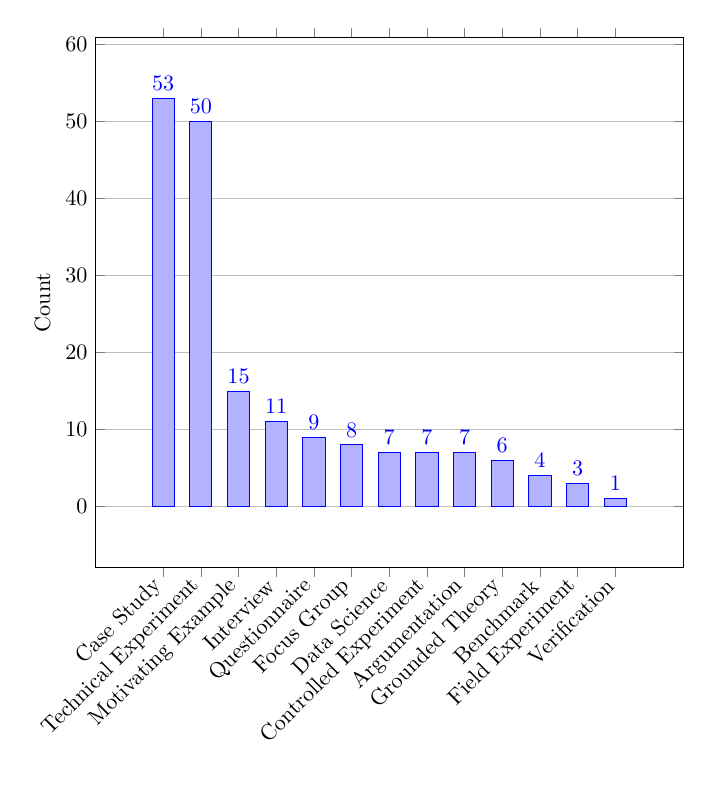
\begin{tikzpicture}[scale=.8]
\begin{axis}[ ybar, ymajorgrids, enlargelimits=0.15, legend style={at={(0.5,-0.15)}, anchor=north,legend columns=-1},
    width=.90\linewidth,height=10cm,
    nodes near coords, %nodes near coords align=below,
    ylabel={Count},ymin=0,
    x tick label style={rotate=45,anchor=east},
    xtick={1,2,3,4,5,6,7,8,9,10,11,12,13},
    xticklabels={Case Study,Technical Experiment,Motivating Example,Interview,Questionnaire,Focus Group,Data Science,Controlled Experiment,Argumentation,Grounded Theory,Benchmark,Field Experiment,Verification 
}
    %xlabel={Evaluation Method}    
    ]
  \addplot coordinates { (1,53)  (2,50)  (3,15)  (4,11)  (5,9)  (6,8)  (7,7)  (8,7)  (9,7)  (10,6)  (11,4)  (12,3)  (13,1)   };
\end{axis}
\end{tikzpicture}
\end{center}
%\caption{Histogramm f\"ur Evaluation Method (188)}
%\label{fig:histo_evaluationmethod}
%\end{figure}

